\documentclass{article}
\usepackage{subfigure}
\usepackage{multicol}
\usepackage{graphicx}
\usepackage[utf8]{inputenc}
\usepackage[margin=.5in]{geometry}
\addtolength{\topmargin}{.875in}
\usepackage{xcolor}
\usepackage{titlesec}
\titleformat{\section}[block]{\color{black}\Large\bfseries\filcenter}{}{1em}{}
\pagestyle{headings}
\markright{blue ball freefall}

\begin{document}

\begin{figure}[h!]
\begin{multicols}{2}
    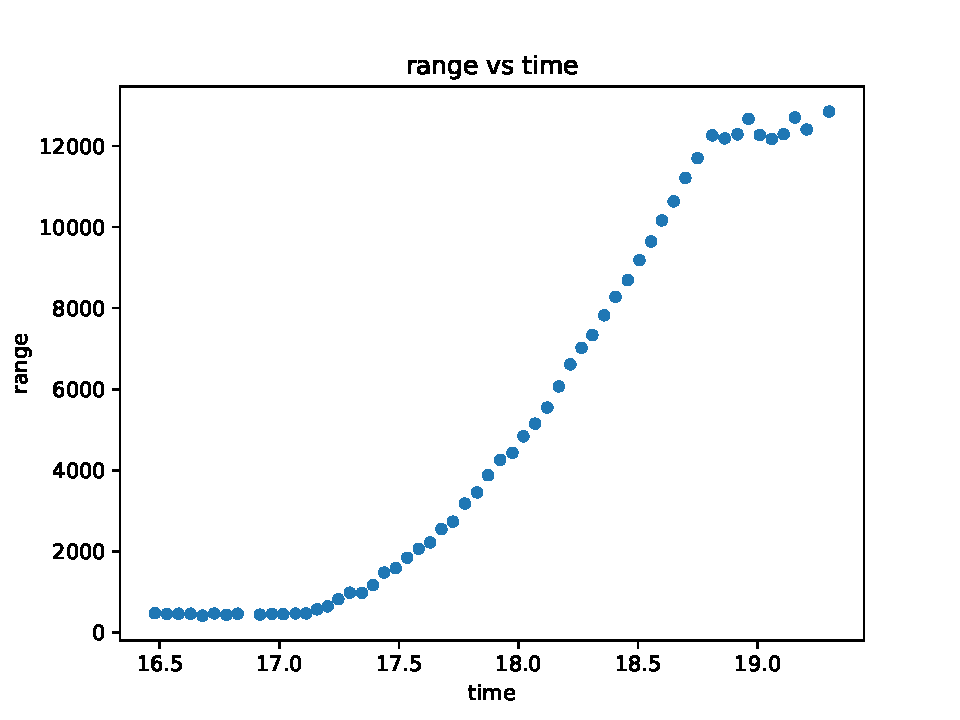
\includegraphics[scale=0.6]{range.pdf}
        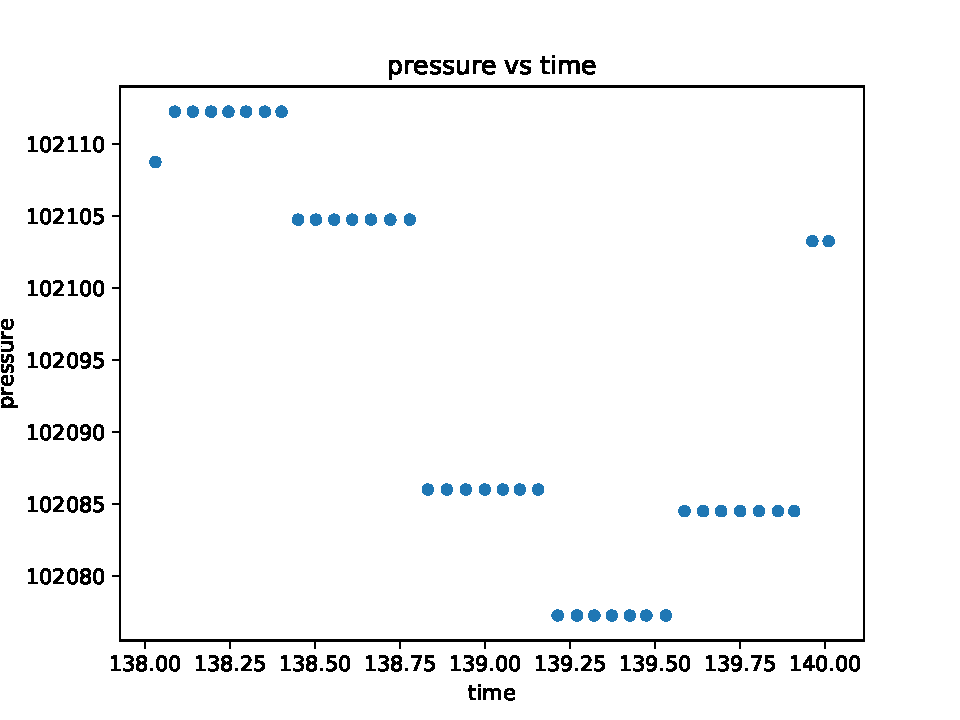
\includegraphics[scale=0.6]{pressure.pdf}
\end{multicols}

\begin{multicols}{2}
    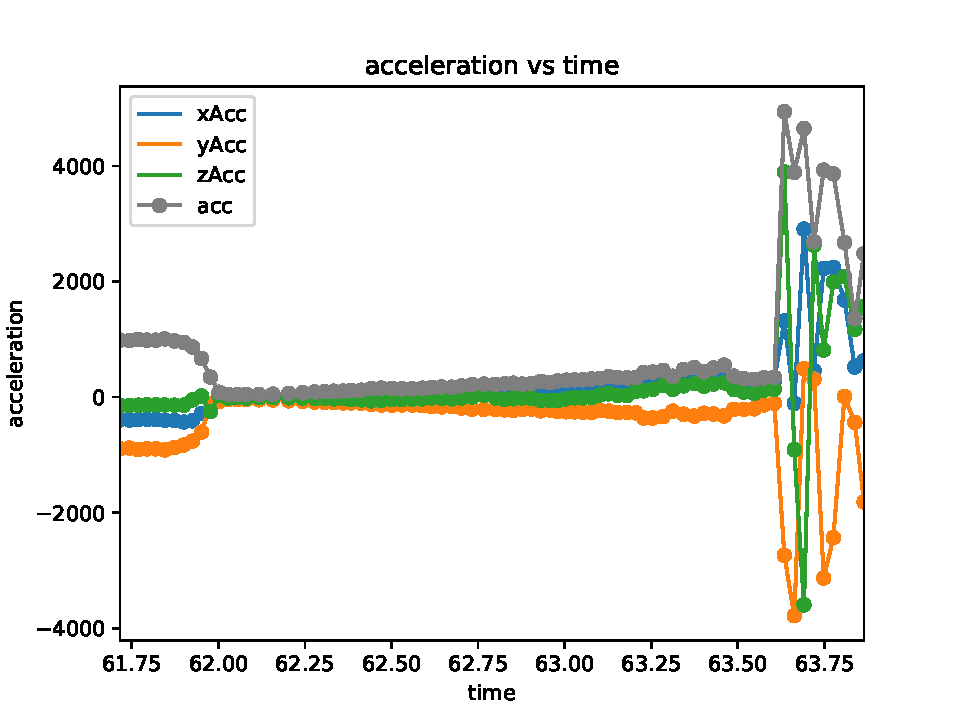
\includegraphics[scale=0.6]{acceleration.pdf}
    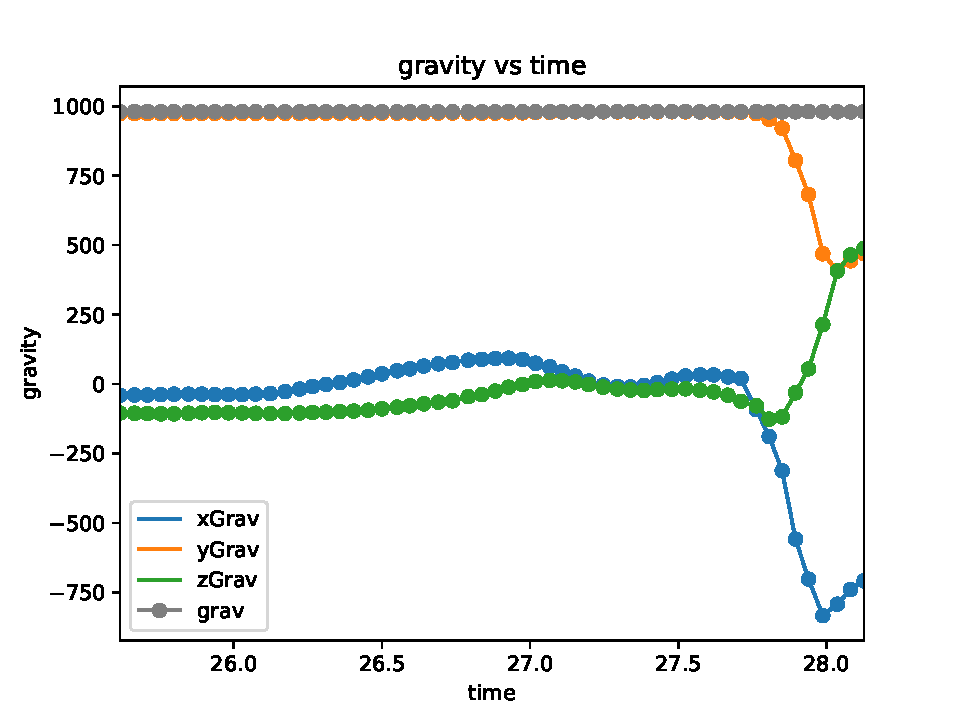
\includegraphics[scale=0.6]{gravity.pdf}
\end{multicols}

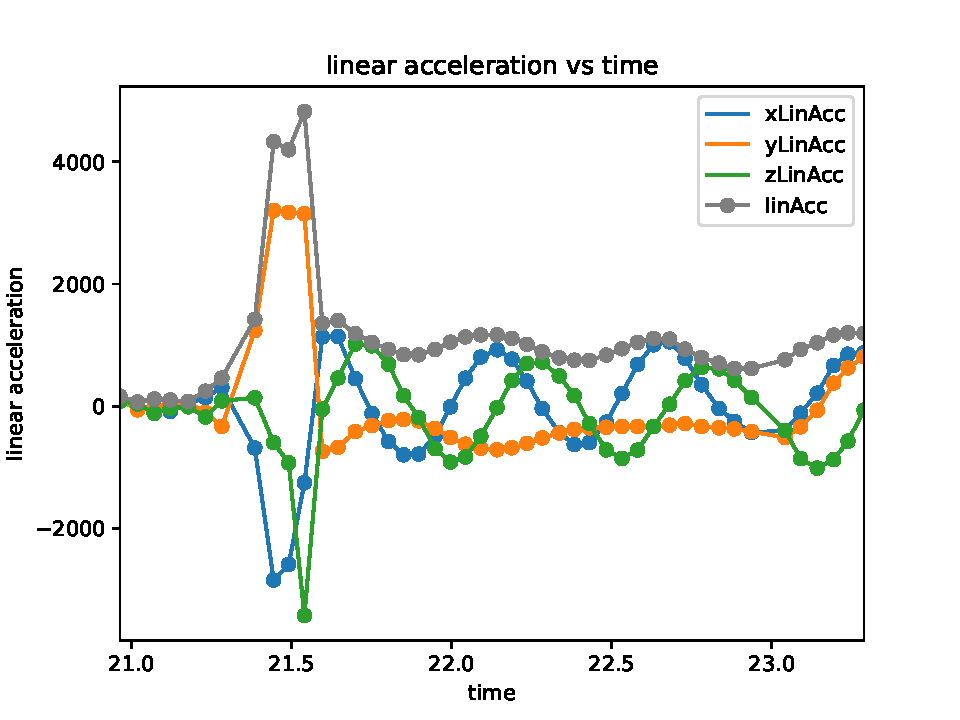
\includegraphics[scale=0.6]{linAcc.pdf}

\end{figure}

\newpage
\begin{figure}[h!]

\begin{multicols}{2}
    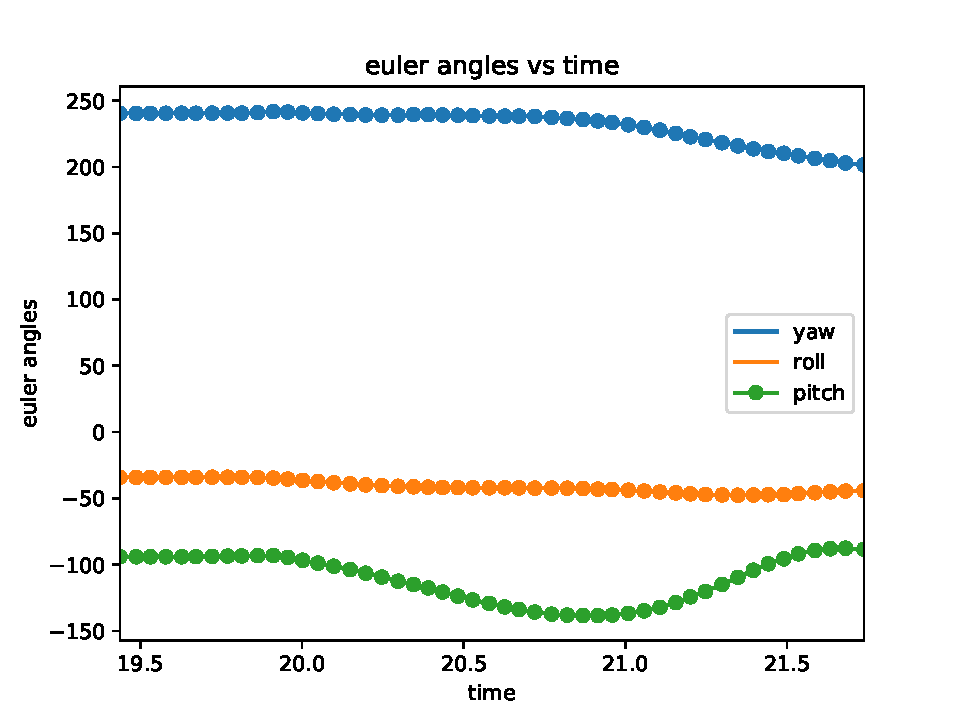
\includegraphics[scale=0.6]{eulerAngles.pdf}
    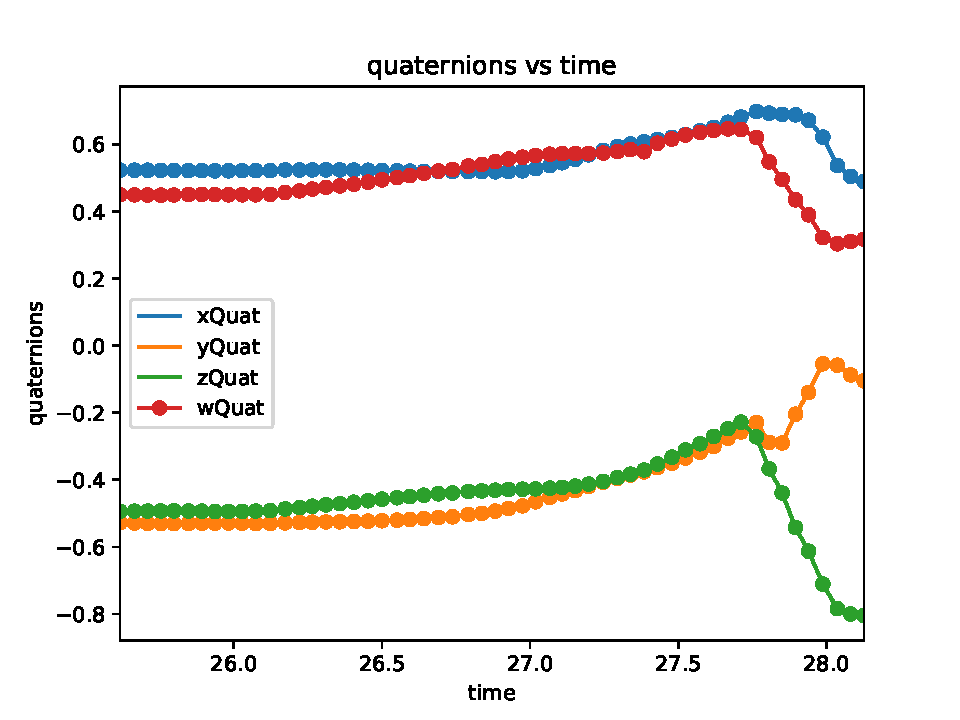
\includegraphics[scale=0.6]{quaternions.pdf}
\end{multicols}

\begin{multicols}{2}
    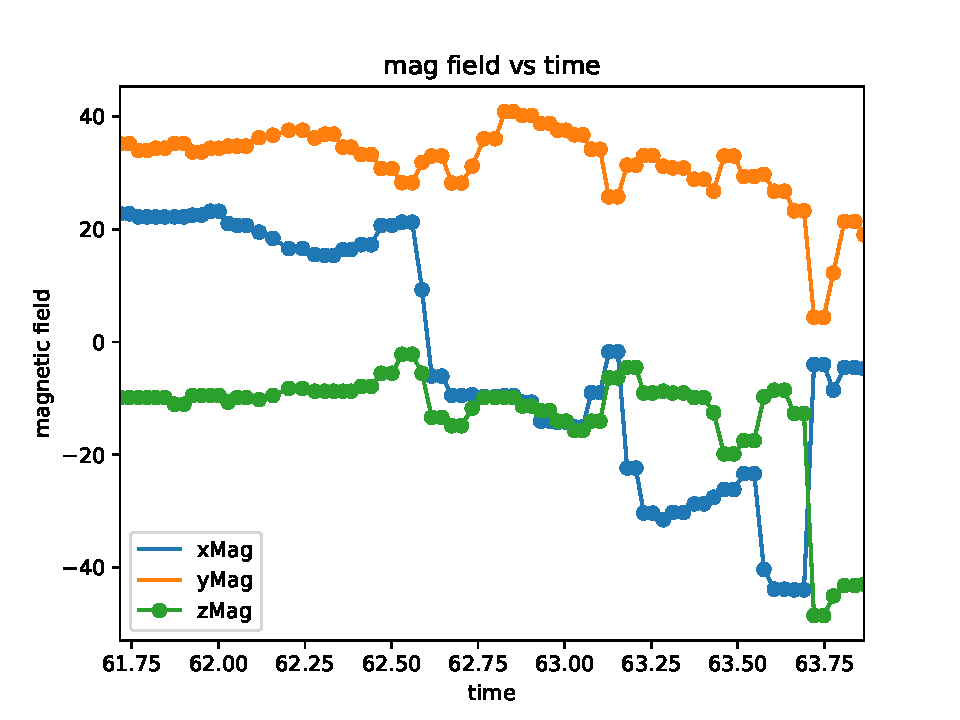
\includegraphics[scale=0.6]{magField.pdf}
    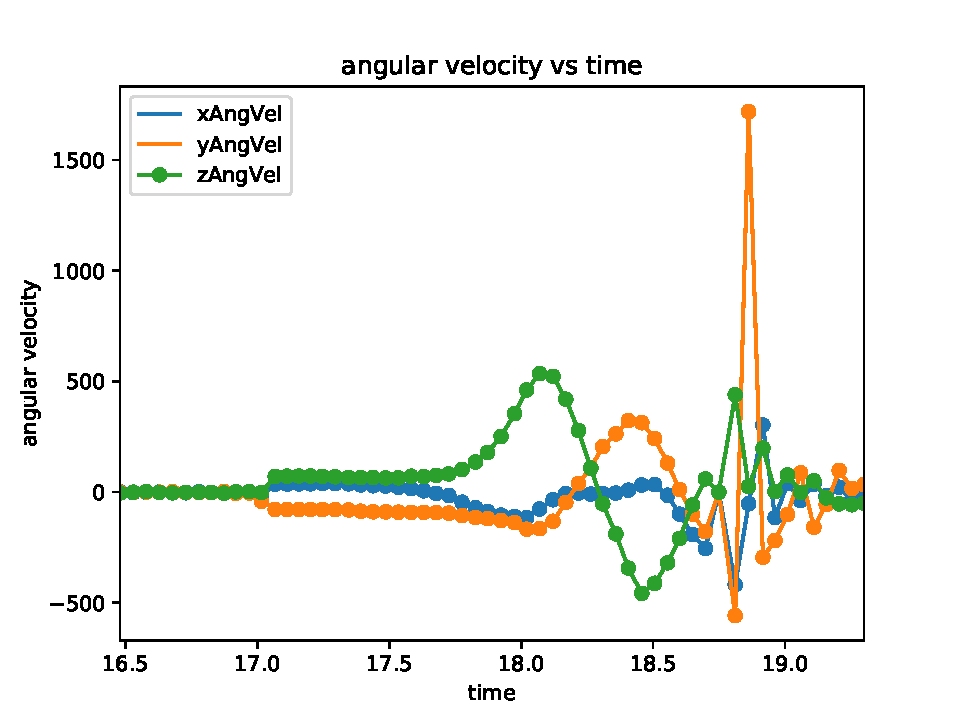
\includegraphics[scale=0.6]{angVel.pdf}
\end{multicols}



\end{figure}

\end{document}
